\documentclass[../Interim_Report_Master]{subfiles}
\begin{document}
\hypertarget{v_and_v}{\section{Verification and Validation of the Existing Code}\label{v_and_v}}
Before the heat and mass transfer methods can be added to the existing code some modifications to it had to be made. The existing code calculates the position and velocity of the particles but also includes a discrete element method (DEM) to simulate the collision of particles. The latter is computationally expensive and is not needed for the heat and mass transfer calculations. The DEM code can be ``switched off'' so the existing code solves just for the particle position and velocity. There are verification and validation checks that need to be done to ensure the modified code is solving the equations correctly and producing physical results.

The cut down code can be found at \cite{andrew_oranges}. 

\subsection{Analytic Test Case}\label{an_test}
One very simple check that can be made initially is to check if results from the code converge to some analytic solution. The ideal test case for this is the droplet accelerating under gravity to reach a terminal velocity. The differential equation to be solved is:
\begin{equation}
\frac{du}{dt} = g + \frac{1}{\tau_d}(u_f-u)
\end{equation}

The full solution procedure can be found in Section \ref{particle_grav_drag_dev}. This leads to:
\begin{equation}
u = \tau_d\left(g + \frac{u_f}{\tau_d}\right)(1-e^{-t/\tau_d})
\end{equation}

To simplify this further the fluid velocity can be set to zero, yielding the simplified formula: 
\begin{equation}
u = \tau_d g(1-e^{-t/\tau_d})
\end{equation}

The settings used for the test case are shown in Table \ref{tab:grav_test_set}:
\begin{table}[h]
	\centering
	\begin{tabular}{|l c|}
		\hline
		\textbf{Parameter} & \textbf{Setting} \\ \hline
		\textbf{Droplet Properties} &  \\ 
		Density of Liquid Phase $\rho_L$ & $997~kgm^{-3}$ \\
		Initial Diameter ${D_0}$ & $0.05~m$ \\ 
		Initial Velocity $u_0$ & $0~ms^{-1}$ \\ \hline 
		\textbf{Gas Properties} &  \\ 
		Kinematic Viscosity $\mu_G$ & $0.1~kgm^{-1}s^{-1}$ \\ \hline
		\textbf{Physical Constants} &  \\ 
		Gravity $g$ & $9.81~ms^{-1}$ \\ \hline
	\end{tabular}
	\caption{Simulation settings used for acceleration under gravity test case.}
	\label{tab:grav_test_set}
\end{table}

For non-dimensionalising the results $\tau_d$ has been used for time and the terminal velocity has been used $u_i$. See Section \ref{sec:term_vel} for a derivation of the terminal velocity formula shown in equation \ref{terminal_v}.
\begin{equation}
v_{final} = u - g\frac{\rho_d D^2}{18\mu_G}
\label{terminal_v}
\end{equation}

Using the settings from Table \ref{tab:grav_test_set} the terminal velocity is:
\begin{subequations}
\begin{align}
v_{final} &= 0ms^{-1} - (9.81ms^{-2})\left(\frac{(997kgm^{-3})(0.05m)^2}{(18)(0.1kgm^{-1}s^{-1})}\right) \\
v_{final} &= -13.58~ms^{-1}
\end{align}
\end{subequations}

Figure \ref{vel_time_tau_4} shows the analytic and numerical solutions for the gravity test case. This shows the particle accelerating to the terminal velocity. As explained earlier, as the numerical solution for the velocity uses an implicit method this under predicts the analytic solution.
\begin{figure}[H]
	\centering
	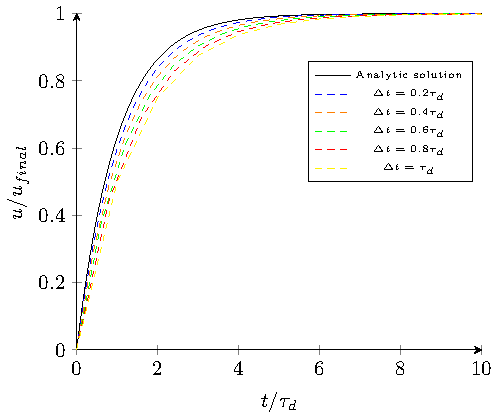
\includegraphics[width=0.8\textwidth]{./Diagrams/Gravity_Verification_Test/Gravity_Verification_Test.pdf}
	\caption{Non-dimensionalised velocity for a droplet sized $D^2=50mm$ with $Re_{d0}=0$, and $\Delta t=\tau_d/2$ and $\Delta t=\tau_d/8$.}
	\label{vel_time_tau_4}
\end{figure}

As with previous tests it is important to check the solution produced by the code converges to the analytic solution. For this test case the simulation time was set as $21$ seconds which is $\sim15\tau_d$. The results from this are shown in Figure \ref{gravity_con}.

\begin{figure}[H]
	\centering
	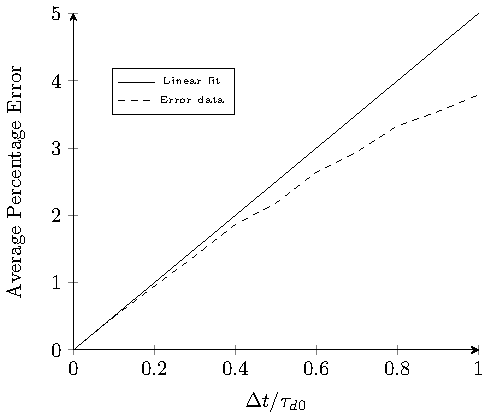
\includegraphics[width=0.8\textwidth]{./Diagrams/Gravity_Verification_Test/Gravity_Convergence/Gravity_Convergence.pdf}
	\caption{convergence of numerical results for gravity test case for a droplet sized $D^2=50mm$ with $Re_{d0}=0$, and a range of timesteps.}
	\label{gravity_con}
\end{figure}

Figure \ref{gravity_con} clearly indicates convergence for the gravity test case. As well as confirming the velocity equation is solved with higher than first order accuracy as reported in \cite{Elijah_GPU_Report}.

\subsection{Statistical Test Case}\label{stat_test_case}
Another check that can be made is to find if the code produces statistically stationary conditions. This can be done by calculating the relative velocity. I.e. the difference between the particle velocity and the fluid velocity at different times. The particle velocity is a Lagrangian variable (only varying with time). Whilst the fluid velocity is an Eulerian variable as it varies with both space and time. To calculate the relative velocity between the particle and fluid a Lagrangian description is needed for velocity.

The averaging procedure to get the relative velocities is:
\begin{subequations}
\begin{eqnarray}
\bar{U}_{x,rel}(t) =& \sum_{i=1}^{N}\frac{\left[U_{p_i}(t)-U_{f_i}(t)\right]}{N} \\
\bar{V}_{y,rel}(t) =& \sum_{i=1}^{N}\frac{\left[V_{p_i}(t)-V_{f_i}(t)\right]}{N} \\
\bar{W}_{z,rel}(t) =& \sum_{i=1}^{N}\frac{\left[W_{p_i}(t)-W_{f_i}(t)\right]}{N}
\end{eqnarray}
\end{subequations}

Where for each velocity component the relative velocity is found for all particles and averaged to produce the mean velocity component. The behaviour of the mean relative velocity will be random initially but should converge to some value at a later point in time. This behaviour should also be the same for the angle between the fluid and particle velocity vectors. 

The Stokes number will dictate the behaviour of the particles. If it is $<<1$ the particles are massless and should follow the flow. If the Stokes number is $>>1$ the particles are essentially billiard balls and the flow field of the velocity has no bearing on the motion of the particles.

The conditions used for the simulation of a Taylor-Green vortex were:
\begin{table}[h]
\centering
\begin{tabular}{|c c|}
	\hline
	\textbf{Parameter} & \textbf{Setting} \\ \hline
	\textbf{Droplet Properties} &  \\ 
	Density of Liquid Phase $\rho_L$ & $2000~kg/m^3$ \\
	Initial Diameter $D_0$ & $0.05~m$ \\ \hline 
	\textbf{Gas Properties} &  \\ 
	Kinematic Viscosity $\mu_G$ & see Table \ref{stk_test_case} \\ 
	Flow Magnitude $A$ & 5 \\
	Vortex Frequency $a$ & 3 \\ \hline
	\textbf{Non-Dimensional Numbers} &  \\ 
	Stokes Number $St$ & see Table \ref{stk_test_case}  \\ \hline
	\textbf{Physical Constants} &  \\ 
	Gravity $g$ & $0~ms^{-1}$ \\ \hline
	\textbf{Simulation Properties} &  \\ 
	Number of Particles & 100 \\ \hline
\end{tabular}
\caption{Simulation settings used for statistical test case.}
\end{table}

\begin{table}[h]
\centering
\begin{tabular}{|c c|}
	\hline
	\textbf{Kinematic Viscosity} & \textbf{Stokes Number} \\ \hline
 	10.40 & 0.1 \\
 	1.04 & 1.0 \\
 	0.1040 & 10.0 \\ \hline
\end{tabular}
\caption{Settings used to get different Stokes numbers.}
\label{stk_test_case}
\end{table}

The distribution of starting conditions gives a mean particle speed of $1ms^{-1}$ and standard deviation of $0.1ms^{-1}$. With the particle directions evenly distributed.

Figure \ref{rel_vel} shows the change in relative velocity between the particles and the fluid. As the Stokes number is increased the particles take longer to respond to the fluid. For a small Stokes number it can be seen that within around 20 momentum relaxation time constants the particle velocity has converged to the fluid velocity. This is further shown by Figure \ref{rel_ang_stk_0_1} where the angle between the particle and fluid velocity converges to zero.

A similar behaviour is present for a Stokes number of 1. However, its takes around twice as long for the relative speeds to converge to zero. By contrast for a Stokes number of 10 the relative speeds and relative angles do not converge at all. This is to be expected as the fluid should have little bearing on the motion of the particles for this Stokes number.
\begin{figure}[H]
	\centering
	\begin{subfigure}[t]{\textwidth}
		\centering
		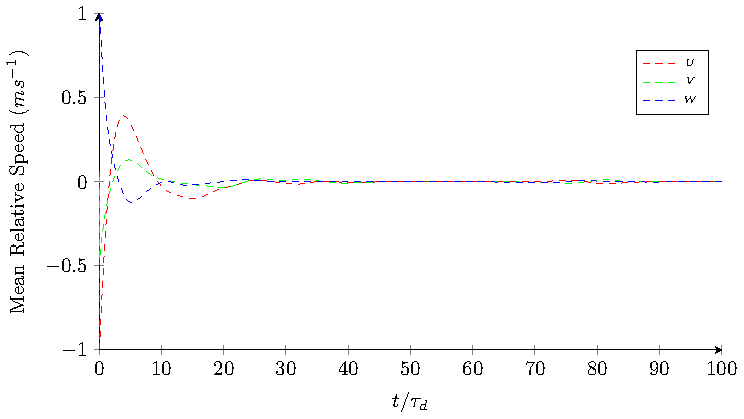
\includegraphics[width=0.8\textwidth]{./Diagrams/Statistical_Verification_Test/stk_0_1/Statistical_Verification_Test_Velocity_stk_0_1_.pdf}
		\caption{Stokes number of 0.1.}
		\label{rel_vel_stk_0_1}
	\end{subfigure}
\end{figure}
\begin{figure}\ContinuedFloat
	\centering
	\begin{subfigure}[t]{\textwidth}
		\centering
		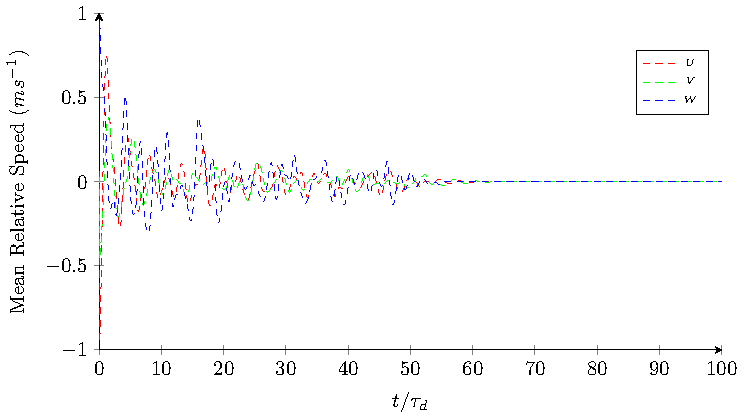
\includegraphics[width=0.8\textwidth]{./Diagrams/Statistical_Verification_Test/stk_1/Statistical_Verification_Test_Velocity_stk_1.pdf}
		\caption{Stokes number of 1.}
		\label{rel_vel_stk_1}
	\end{subfigure}
\end{figure}
\begin{figure}\ContinuedFloat
	\centering
	\begin{subfigure}[t]{\textwidth}
		\centering
		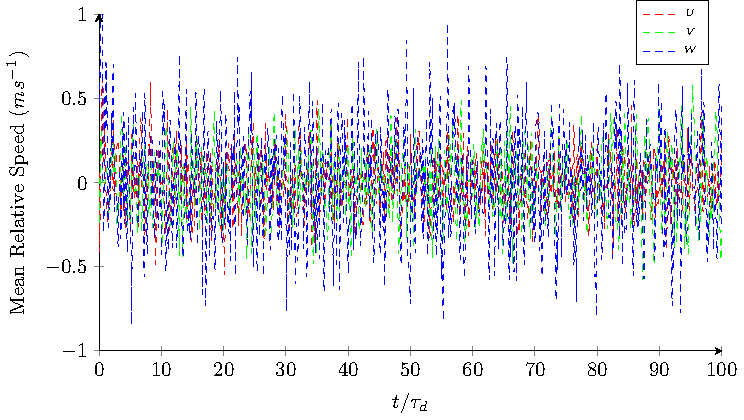
\includegraphics[width=0.8\textwidth]{./Diagrams/Statistical_Verification_Test/stk_10/Statistical_Verification_Test_Velocity_stk_10.pdf}
		\caption{Stokes number of 10.}
		\label{rel_vel_stk_10}
	\end{subfigure}
\caption{Plots of mean relative speed between the particle and fluid for each velocity component for Stokes numbers of 0.1 (a), 1.0 (b) and 10 (c).}
\label{rel_vel}
\end{figure}

\begin{figure}[H]
	\centering
	\begin{subfigure}[t]{\textwidth}
		\centering
		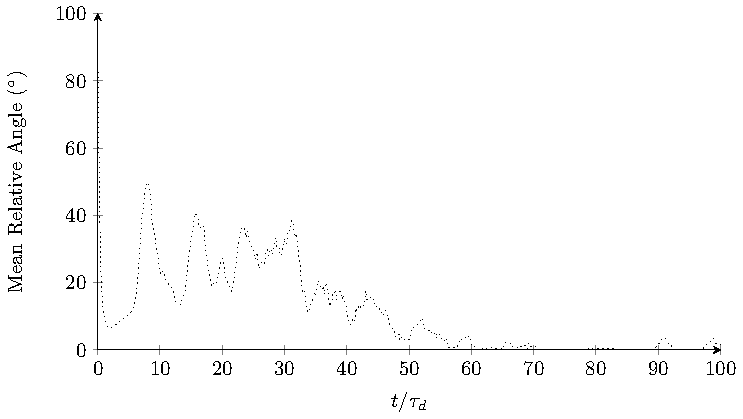
\includegraphics[width=0.8\textwidth]{./Diagrams/Statistical_Verification_Test/stk_0_1/Statistical_Verification_Test_Angle_stk_0_1_.pdf}
		\caption{Stokes number of 0.1.}
		\label{rel_ang_stk_0_1}
	\end{subfigure}
	\begin{subfigure}[t]{\textwidth}
		\centering
		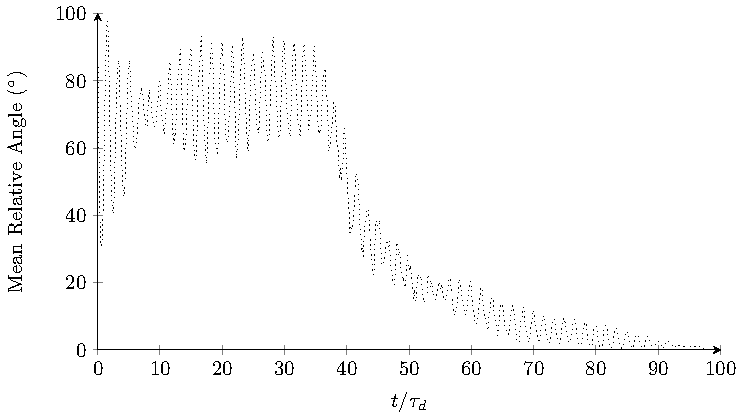
\includegraphics[width=0.8\textwidth]{./Diagrams/Statistical_Verification_Test/stk_1/Statistical_Verification_Test_Angle_stk_1.pdf}
		\caption{Stokes number of 1.}
		\label{rel_ang_stk_1}
	\end{subfigure}
	\begin{subfigure}[t]{\textwidth}
		\centering
		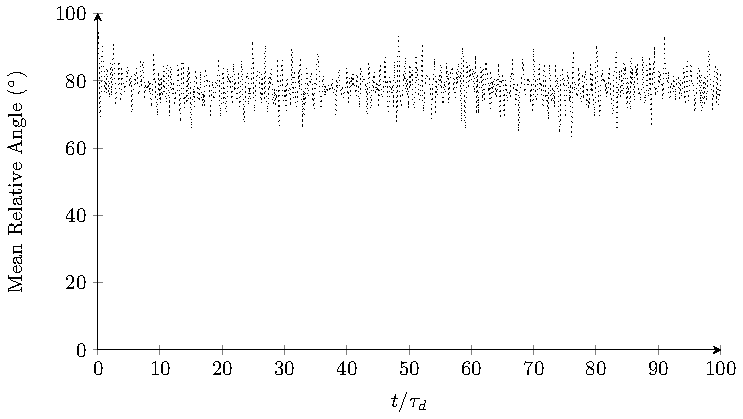
\includegraphics[width=0.8\textwidth]{./Diagrams/Statistical_Verification_Test/stk_10/Statistical_Verification_Test_Angle_stk_10.pdf}
		\caption{Stokes number of 10.}
		\label{rel_ang_stk_10}
	\end{subfigure}
	\caption{Plots of mean relative angle between the particle and fluid velocity vectors for Stokes numbers of 0.1 (a), 1.0 (b) and 10 (c).}
	\label{rel_ang}
\end{figure}

\subsection{Run Time Test}
A final check on the existing code is to measure the run time. As the code uses first order numerical methods and runs on a GPU the run time of the code as a function of the number of particles should be linear.

\begin{figure}[H]
	\centering
	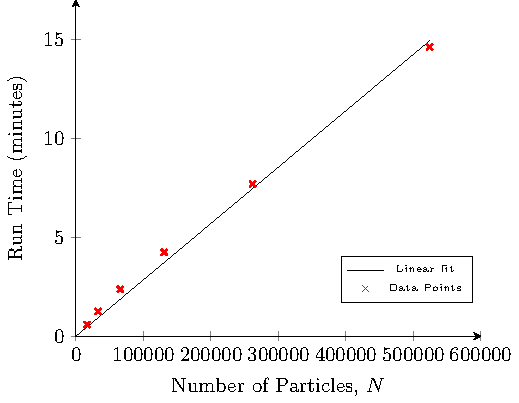
\includegraphics[width=0.8\textwidth]{./Diagrams/Timing/Oranges_Time_Test.pdf}
	\caption{Run time of OpenCl code without data logging for different numbers of particles.}
	\label{oranges_time_test}
\end{figure}

Figure \ref{oranges_time_test} shows the results from this testing. For low numbers of particles the run time is not linear as the initialisation process is a large percentage of the overall simulation run time. However, for a larger number of particles this is no longer the case. 

This set of results provides a point of comparison for when the heat and mass code is added. It should be expected that as first order methods for the heat and mass transfer equations have been used the run time of the code should still be linear. 

\subsection{Problems Encountered with the Existing Code}
Listed in this section are bugs and problems encountered with the existing code. Bugs encountered were found by the author and fixed by E. Andrews with exception of the logstep issue. The full history of the code can be found at \cite{andrews2020}.

\subsubsection{Periodic Boundary Condition}
One misstep that was made in cutting down the existing code was removing the boundary condition for the particle location. The simulation domain is a cube; when a particle reaches the edge of the boundary its position is reset at the other side of the boundary as shown in Figure \ref{periodic_boundary}.
\begin{figure}
	\centering
	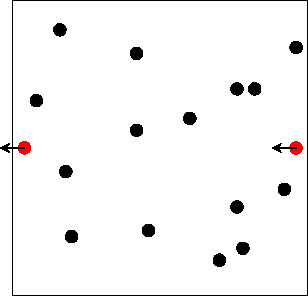
\includegraphics[width=0.5\textwidth]{./Diagrams/Periodic_Boundary/Periodic_Boundary.pdf}
	\caption{Diagram of a periodic boundary implementation.}
	\label{periodic_boundary}
\end{figure}

This is a periodic boundary condition and ensures all the particles remain with the cube. Removing this boundary condition means the particles exit the domain at some velocity vector which remains unchanged as it is no longer influenced by the fluid. 

\subsubsection{Memory Alignment of Structures}
The second issue encountered was adding a variable to the particle structure to record the fluid velocity. To ensure consistency between the host code and device code, structures passed to the device should be aligned. This means setting the order of the variables in the structure from the largest data type to the smallest. It also means for using a gcc compiler telling the compiler the required size of the structure. This is the size of the structure that fits within the smallest power of 2. For example, the size of the particle structure with the added variable can be determined from summing the size of the individual data types.
\begin{table}[h]
\centering
\begin{tabular}{|l c c c|}
	\hline
	\multicolumn{1}{|c }{Data Type} & Size (bytes) & No. of & Total Size (bytes) \\ \hline
	cl\_float3 & 12 & 5 & 60\\
	cl\_ulong & 8 & 2 & 16 \\ 
	cl\_float & 4 & 4 & 16\\ \hline
\end{tabular}
	\caption{Data types and their respective sizes for the OpenCL language.}
\end{table}

This gives a total size for the structure as 92 bytes. The next highest power of 2 is 128 so this is the size of the structure specified. For MSCV compilers the same value is used but the amount of padding must also be specified. This is the size specified minus the actual size. (In this case 36 bytes). 

\subsubsection{File Directory Checking}
The code performs a number of tests during the setup of the simulation to prevent subsequent errors occurring. 

To output the results of the simulation the code writes a text file at some user defined ``log step''. For the logging to work the program needs to know an accessible logging directory exists. It must therefore check this is the case. 

When compiled with MSVC the code performs the check using \lstinline[style=cstyleintext]|GetFileAttributes| as in Figure \ref{code:dir_check_msvc}.
\begin{figure}[h]
\begin{lstlisting}[frame=single, style=cstyle]
if (GetFileAttributes(dir) == INVALID_FILE_ATTRIBUTES) {
	return FALSE;
} else {
	return TRUE;
}
\end{lstlisting}
\caption{Check to see if logging directory exists with \lstinline[style=cstyleintext]|GetFileAttributes|.}
\label{code:dir_check_msvc}
\end{figure}

When compiled with gcc the code checks if the directory exists by trying to open and close the directory as shown in Figure \ref{code:dir_check_gcc}.
\begin{figure}[h]
\begin{lstlisting}[frame=single, style=cstyle]
DIR *dir_obj = opendir(dir);
if (dir_obj) {
	/* Directory exists. */
	closedir(dir_obj);
	return TRUE;
} else if (ENOENT == errno) {
	/* Directory does not exist. */
	return FALSE;
} else {
	/* opendir() failed for some other reason. */
	return FALSE;
}
\end{lstlisting}
\caption{Check to see if logging directory exists.}
\label{code:dir_check_gcc}
\end{figure}

Originally the code used the \lstinline[style=cstyleintext]|stat| structure to perform this check which only worked correctly on some Windows computers.

\subsubsection{Initialisation of Particle Speeds}
The code uses a Box-Muller transformation to turn uniformly distributed random numbers into a normal distribution for initialisation of particle speeds. 

The process is as follows:
Generate two random numbers $u$ and $v$ between $0$ and $1$ using \lstinline[style=cstyleintext]|rand| and \lstinline[style=cstyleintext]|RAND_MAX| as per Figure \ref{code:uv_gen}.
\begin{figure}[h]
\begin{lstlisting}[frame=single, style=cstyle]
u = (float) rand() / (float) (RAND_MAX);
v = (float) rand() / (float) (RAND_MAX);
\end{lstlisting}
\caption{Creation of $u$ and $v$.}
\label{code:uv_gen}
\end{figure}

Next, the normal distribution parameters (mean $\mu$ and standard deviation $\sigma$) must be specified. Then the normal distribution of speeds using the Box-Muller transform are created using:
\begin{equation}
speed = \sigma \sqrt{-2\ln(u)} \cos(2\pi v) + \mu
\end{equation}

This formula is problematic in that it contains a log. If $u$ is set to zero then $\ln(u)$ will tend to $-\infty$. This only occurred for two particles in a population of $100,000$ particles. This does not affect the other particles but prevented Paraview from being able to read the text files produced by the code. The fix was to add $1$ to the random numbers as in Figure \ref{code:uv_fix} so that $u$ and $v$ can not be zero.
\begin{figure}[h]
\begin{lstlisting}[frame=single, style=cstyle]
u = (float) (rand() + 1) / (float) (RAND_MAX + 1);
v = (float) (rand() + 1) / (float) (RAND_MAX + 1);
\end{lstlisting}
\caption{Ensuring $u$ and $v$ can not be zero.}
\label{code:uv_fix}
\end{figure}

\subsubsection{Logsteps Being Skipped}
The Python implementation of the code logs data at the end of every timestep. This solution is fine for one particle but not is not suitable when considering thousands of particles as the amount of data generated would be very large. The OpenCL code includes a logstep which determines how frequently data is logged. This means small timesteps can be used to increase accuracy and logsteps can be set larger than the timestep to reduce the amount of data generated.

The code responsible for this is contained within the main time loop of the simulation as presented in Figure \ref{code:log_loop}.
\begin{figure}[h]
\begin{lstlisting}[frame=single, style=cstyle]
if (LOG_DATA && time - last_write >= log_step) {
	ret = particlesToHost(queue, gparticles, &hparticles, NUMPART);
	printf("Logging at time: %f nn", time);

	if (!writeParticles(hparticles, time, prefix, log_dir, NUMPART, log_vel)) {
		return 1;
	}
	
	last_write = time;
}
\end{lstlisting}
\caption{Determining if data is logged during the timestep.}
\label{code:log_loop}
\end{figure}

The boolean \lstinline[style=cstyleintext]|LOG_DATA| is used to determine if data is to be logged or not. The second part of the condition is the current time subtract the time data was last written must be greater than or equal to the log step. For some values the second part of the if statement would not return true even when this should have been the case. (This is most likely a rounding error). Putting a ``fudge factor'' of $0.99$ on the logstep as shown in Figure \ref{code:log_data_fix} fixed this problem.
\begin{figure}[h]
\begin{lstlisting}[frame=single, style=cstyle]
if (LOG_DATA && time - last_write >= 0.99*log_step) {
\end{lstlisting}
\caption{Data logging fix.}
\label{code:log_data_fix}
\end{figure}
\end{document}


